\documentclass[runningheads]{llncs}
%
\usepackage[T1]{fontenc}
\usepackage{graphicx}
\usepackage{tikz}
\usepackage{wrapfig}
\usepackage{package/mathpartir}
\usepackage{todonotes}
\usepackage{xspace}

\usepackage{package/regles}
\usepackage{mathtools}
\usepackage{ amssymb }

\usepackage{package/formal-grammar}
\usepackage{package/mathpartir}

\newcommand{\Nat}{{\mbox{$\mathbb{N}$}}}
\newcommand{\tuple}[1]{\ensuremath{\langle #1\rangle}}

\newcommand{\directions}{\dirFmt{\mathsf{D}}}
\newcommand{\internalState}{{\mathcal{I}}}

% Je suis assez d'avis de distinguer la direction des blocks et des trains
\newcommand{\forward}{\ensuremath{\mathtt{f}}}
\newcommand{\backward}{\ensuremath{\mathtt{b}}\xspace}
\newcommand{\sucblock}{{\mathtt{suc}}}
\newcommand{\networkConf}{\ensuremath{\Sigma}}

%% Train directions
\definecolor{dircolor}{rgb}{1.0, 0.13, 0.32}
\newcommand{\dirFmt}[1]{{\color{dircolor}{#1}}}
\newcommand{\dirForward}{\ensuremath{\dirFmt{\forward}}\xspace}
\newcommand{\dirBackward}{\ensuremath{\dirFmt{\backward}}\xspace}
\newcommand{\dirStop}{\ensuremath{\dirFmt{\star}}\xspace}

%% Positions
\definecolor{poscolor}{rgb}{0.6, 0.45, 0.32}
\newcommand{\posFmt}[1]{{\color{poscolor}{#1}}}
\newcommand{\blocks}{{\posFmt{\mathsf{B}}}}
\newcommand{\bid}[1]{\posFmt{b_{#1}}}

%% Switches
\definecolor{swcolor}{rgb}{0.4, 0.23, 0.56}
\newcommand{\swFmt}[1]{{\color{swcolor}{#1}}}
\newcommand{\sid}[1]{\ensuremath{\swFmt{s_{#1}}}}
\newcommand{\turnouts}{\swFmt{\mathsf{\theta}}}

%% Trains
\definecolor{traincolor}{rgb}{0.2, 0.2, 0.6}
\newcommand{\trainFmt}[1]{{\color{traincolor} #1}}
\newcommand{\trainTuple}[4]{\langle \trainFmt{#1}, \posFmt{#2}, \dirFmt{#3}, #4 \rangle}
\newcommand{\trainSeq}{\trainFmt{\Gamma}}
\newcommand{\trains}{{\trainFmt{\mathsf{T}}}}
\newcommand{\tid}[1]{\ensuremath{\trainFmt{t_{#1}}}}

%% Regulator's Program
\newcommand{\regTuple}[3]{\tuple{#1, #2, #3}}
\newcommand{\evGuard}[2]{\ensuremath{\mathtt{ev}(\trainFmt{#1}, #2)}}
\newcommand{\ev}[3]{\evGuard{#1}{#2}: #3}
\newcommand{\incr}[1]{{\mbox{\ensuremath{\mathtt{incr}(\posFmt{#1})}}}\xspace}
\newcommand{\turn}[2]{{\mbox{\ensuremath{\mathtt{turn}(#1, #2)}}}\xspace}
\newcommand{\tokens}{\ensuremath{T}}
\newcommand{\tokenOf}[1]{\ensuremath{T(\posFmt{#1})}}


%% Signals
\newcommand{\sigred}{{\mbox{${\color{red!50!black}\mathtt{r}}$}}\xspace}
\newcommand{\siggreen}{{\mbox{${\color{green!50!black}\mathtt{g}}$}}\xspace}
\newcommand{\deviate}{{\mbox{$\mathtt{v}$}}\xspace}
\newcommand{\direct}{{\mbox{$\mathtt{d}$}}\xspace}
\newcommand{\signalF}[2]{\ensuremath{F(\posFmt{#1}, \dirFmt{#2})}}

%% Reduction relation
\newcommand{\reduces}{\ensuremath{\rightarrow}}

%% tt style

\newcommand{\su}[2]{{\mbox{$\mathtt{startuntil}(\dirFmt{#1}, \posFmt{#2})$}}\xspace}




\begin{document}
%
\title{A formal approach but practical approach in train regulation}
%
%\titlerunning{Abbreviated paper title}
% If the paper title is too long for the running head, you can set
% an abbreviated paper title here
%
\author{Lucas Villaume \and Guillaume Bonfante \and Martin Vassor  }
%
\authorrunning{L. Vuillaume et al.}
% First names are abbreviated in the running head.
% If there are more than two authors, 'et al.' is used.
%
\institute{Université de Lorraine -- CNRS -- INRIA -- LORIA}
%
\maketitle
%
\begin{abstract}
	% Contexte
	Trains networks are critical system which failure may lead to numerous fatalities, in case of crashes, or important loss, if trains are not properly routed. 
	% Problème
	In this paper, our goal is to formally verify the correctness of train routes. More precisely, we verify the absence of deadlocks, the termination, and the absence of crashes.
	% Approche
	To address this question, we model train systems in TLA+. Our model includes trains, as well as switches, detection sensors and traffic lights. Both switches and traffic lights are controlled by a regulator upon train events. We provide trains and the regulator lists of event, which characterise the train scheduling, which is then checked using TLA+'s model checker.
	% Resultats
	Our contributions are threefold: first, we provide a TLA+ specification which can be adapted to various train networks and schedules; second, we report tests we ran on the model on a non-trivial network, composed of 3 trains, 8 blocks and 5 switches; finally we show how to sequentially compose two schedules and to verify the result.

\keywords{First keyword  \and Second keyword \and Another keyword.}
\end{abstract}


\section{Introduction}
\label{sec:introduction}

This contribution finds its origin in a cyber-warefare we are organising for students at the University of Lorraine concerned by cyber-security, see~\cite{CHE}. In the game-play, we have both IT infrastructures and physical systems, with connections between them. On the physical side, we built a small train network that tries to be a good model of real systems.  Our system manages customer informations, train regulation and finally the physical/infrastructure layer. Attackers can hit any of the three parts: disfiguring the website, changing a platform or blocking a signal. Defenders will protect their system, typically via a strict network policy.

\medskip

\begin{wrapfigure}[6]{r}{0.45\textwidth}
\vspace{-6mm}
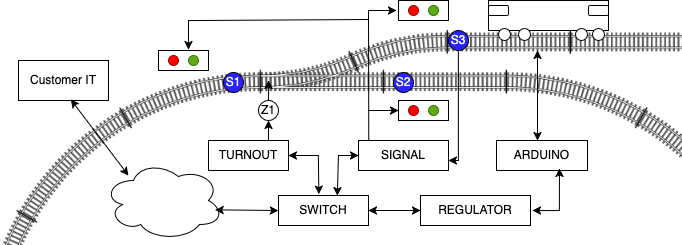
\includegraphics[height=20mm]{TrainSchema.png}
\end{wrapfigure}


From an Information Technology (IT) point of view, our system is shaped as shown on the right. Switches are controlled by a raspberry (TURNOUT) running an OpenPLC program, signals are controlled by an other raspberry, SIGNAL, with access to turnout positions via modbus. Then, the SIGNAL PLC reads mouvement sensors  (not all links shown in the figure) to update the status of signals. Next to that, we have a third machine, the regulator: it is in charge of updating train routes (as required by the customer IT),  of the regulation of turnouts and finally it may lock some signal (turn it to "red"). All the network connections are done via a single switch. Connections from REGULATOR to TURNOUT and SIGNAL are done via modbus while the customer IT and the regulator exchanges  are based on TCP/IP.  To be complete, to activate train mouvements, we use the DCC protocol via an Arduino, but this part is strictly related to the fact we have a train model. 


\begin{wrapfigure}[7]{r}{0.3\textwidth}
\hspace{-10mm}
 \begin{minipage}{0.3\textwidth}
        \centering
        \vspace{-24mm}
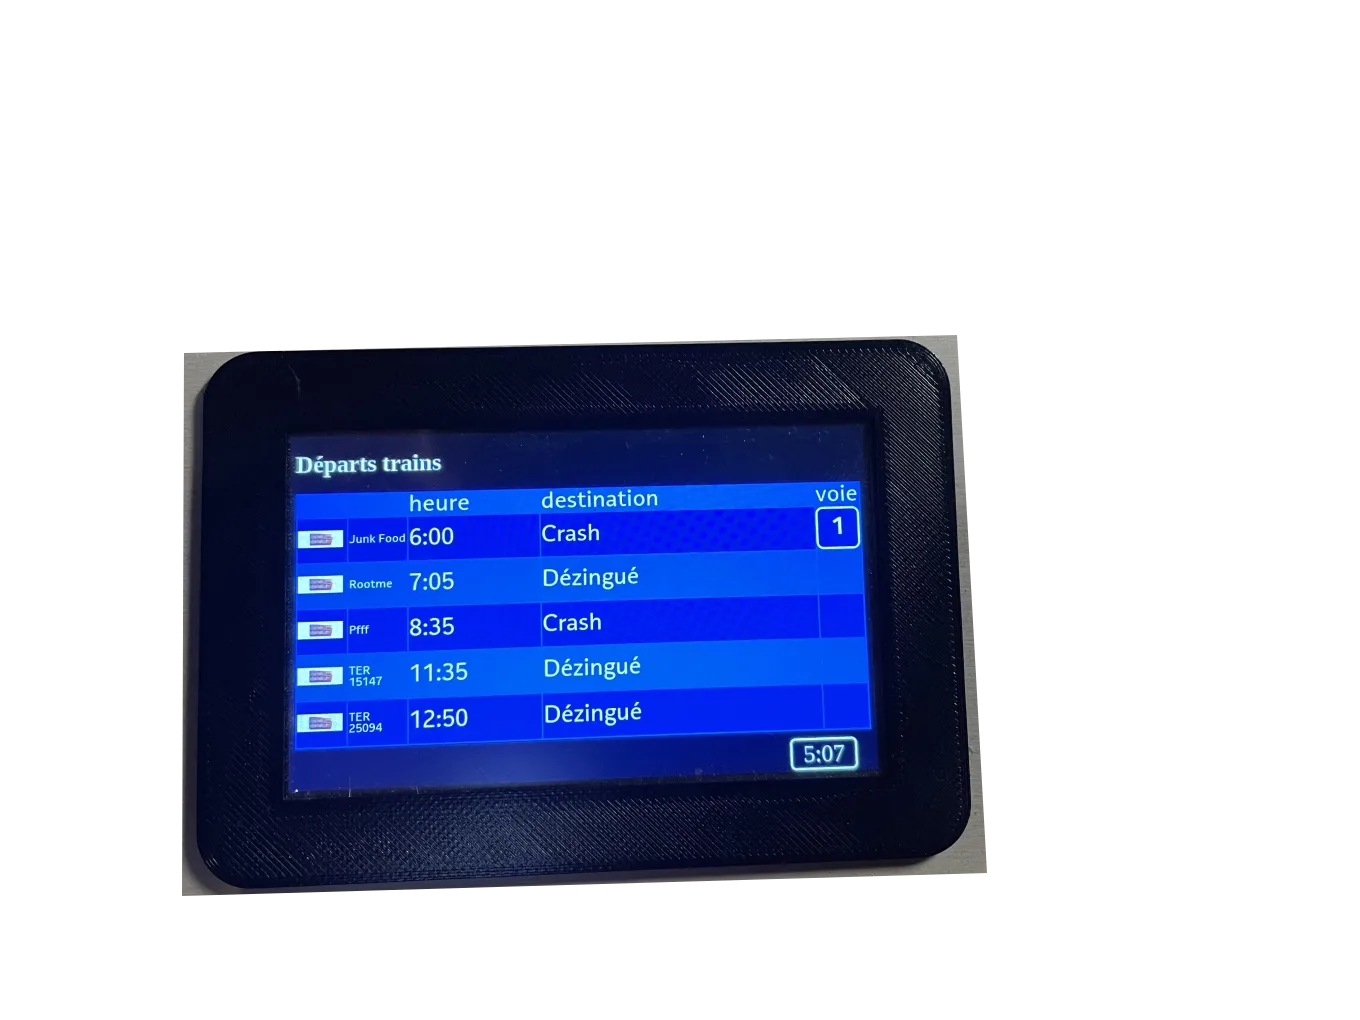
\includegraphics[height=50mm]{ZoomAffichage.png}
    \end{minipage}
\end{wrapfigure}

 The customer IT is deported from the infrastructure IT (thus the cloud).  It is itself composed of three machines: one for the station screens (on the right, after an attack), one for the databases and a final orchestrator. On the orchestrator, there are two main services: we have a web-service (with front and backend) and the general route scheduler.  Our model is completely automatic, no manual intervention is needed apart from minor electrical/mechanical problems that come with our scale model.
 
\begin{wrapfigure}[8]{r}{0.28\textwidth}
 \begin{minipage}{0.28\textwidth}
        \centering
        \vspace{-8mm}
\includegraphics[height=30mm]{maquette.png}
    \end{minipage}
\end{wrapfigure}

\paragraph{Final words on the N-scale model.} Our circuit has 8 blocks, 5 switches. Each block is bidirectional with a signal at each end. Blocks size goes from 25cm to 70cm.  We operate  three trains in parallel. Due to the size of the model, we reduced our signals  to "red" and "green" status, the trains being too close one from the other. Furthermore, in case of a red signal, we make the hypothesis that the train will be able to stop before it reaches the end of the block. In practice, we stop the trains in the middle. 

\paragraph{Routing trains.}
\todo{Ajouter: tout est automatique}
Routes are computed on the fly. The schedule is renewed every "day"\footnote{We use a time scale factor: one of our "day" corresponds to 20 minutes in real time.}  and we introduce some randomness in the process: beyond some routine daily planning, some trains are inserted/deleted, some trains departure/destination may change, and so on. We simulate also delays. Finally, in our model, we distinguish freight and  passengers routes giving priority to the latter. Routes are recomputed each time a train has finished its duty. The general motivation of this paper is to propose a lightweight scheduling solution that is adapted to the fully automatic control, that takes into account the distributed nature of the system, that is reliable and does not suffer from interlocking.  
 
We can now describe in more detail the working assumptions we are making about planning.  First, we have sensors on the rails at the two ends of each block. Accordingly,  we can catch train entrances within blocks. We make the hypothesis that this task is performed without errors. Second, the switches can be swapped from one position to the other, again, we suppose it is done without fault. Our method could cope such issues, but we leave that for future work. 
 
  Third, for trains, we have a simple policy.  According to its plan, a train may start in some direction (Forward/Backward) up to some final position. Then, once started, the train will run according to the signals: when green, it (re-)starts, when red, it stops.  We do not make hypotheses on the durations of travels, but once a train is running, it will reach in finite time the next block. Trains run in parallel independently. One train may enter a block, while an other is crossing some switch and the third one is breaking. There is no communications between the trains.

Fourth,  the regulator is capable of reading train block entrance events, requiring some switch swap and finally locking (that is make sure a signal is red)/unlocking some signal. We consider that those latter operations can be carried out without delay. Finally, the regulator may append some new duty to a train. To sum up, to control the train mouvements, the regulator can only lock/unlock signals. Naturally, a signal intended to block train $T_1$ may block $T_2$ if not set at the right time.   
 
 Parler de la stratégie, du modèle générale. All these operations are done by what we call  \emph{orders}. Roughly speaking, trains Orders have the shape "Start in direction Until position". Regulator orders are: \todo{en parler}. 
 
 
 To sum up, the regulation policy can be seen as an asynchronous distributed system. The N trains and the regulator are independent agents. That led us to TLA+, a framework introduced by Leslie Lamport for these kind of problems~\cite{Lamport}.  
 
\todo{ Comparaison avec les travaux antérieurs / lit review}
 
 
Due to the distributed nature of the regulation, building a safe policy can be very tricky. We want to show in this paper that tools from formal methods are very useful in this respect.  In this paper, we describe in  a first step the formalisation process. We go up to a TLA+ specification that will allow us checking two properties of route orchestration: safety and liveness. This is our first research question. 

Our second research question is the related to the following need. Suppose we want to append a new duty once a train reached its destination. This can be formalised as a composition problem (how to compose/concatenate some routes with some others). We describe such a composition procedure and then, again, we check that the routes are both safe and deadlock free. 

For our last research problem, we show that TLA+ may be used to refine a regulation policy. In our first attempts, we had typically some deadlocks issues. We have been able to detect them via TLA+ and then to provide some correction. 


% ############################# %
% Espace réservé aux encadrants %
% ############################# %


\subsection{Notations}

Given some set $S$ and some $x \not\in S$, we denote by $S_x = S \cup \{ x\}$.  An other notation: given some function $f: X \to Y$, $x \in X$ and $y \in Y$, we denote by $f[x \leftarrow y]$, the function:
 $$f[x \leftarrow y] \triangleq \left\{  \begin{array}{ll} x &\mapsto y\\
x' \neq x \in X &\mapsto f(x')
\end{array}\right.$$


\section{Model configurations}
\label{sec:informal-model}

In this section, we present configurations of our model, i.e. how we represent, at a given point in time, the state of our network. The dynamic rules of train routing are then presented in the following section.

Our model is has $k+1$ agents corresponding to the $k$ trains and the Regulator. Those agents take place on an infrastructure consisting of a track network equipped with signals. We first present the infrastructure model, then the agents.

\subsection{Infrastructure}

\paragraph{The network.} 

We suppose that the train network can be described as follows. First, we consider a set of $n$ blocks: $\blocks = \{ \bid{1}, \bid{2}, \ldots, \bid{n}\}$. Blocks are oriented: there is a $\dirForward$ (forward) end and a $\dirBackward$ (backward) one. Let $\directions = \{\dirForward, \dirBackward\}$ be the set of directions.  Second, we consider a set of $m$ trackworks\footnote{For the sake of simplicity, in this paper, we only consider switches. Our work can easily be extended to crossings and double slip switches (e.g. crossings have only one internal state and double slip switches have four states).}: $\turnouts = \{\sid{1}, \ldots, \sid{m}\}$. Trackworks are characterized by an internal state: switches can be in direct or deviate position (next denoted '\direct' and '\deviate'). Let $\internalState$ denotes the set of internal states. A \emph{network configuration} is given by a function $\sigma: \turnouts \to \internalState$. Let $\networkConf$ denotes the set of all network configurations. For instance, for two turnouts $\theta = \{\sid{1}, \sid{2}\}$, the function $\sid{1} \mapsto \deviate, \sid{2} \mapsto \direct$ states that switch $\sid{1}$ is in deviate position while \sid{2} is in direct one. The latter function is also described via an array  $[\deviate, \direct]$ giving states in trackwork order. 

The network is then described as a triple $(\blocks, \turnouts, \sucblock)$ where $\sucblock$ is a partial function indicating the following block given a starting position, a direction and a network configuration: $\sucblock: \blocks\times \directions \times \networkConf \to \blocks$. We note $\sucblock(pid, d, \sigma) = \bot$ when it is undefined. From an abstract point of view, the topology of the network reduces to that data.  


\paragraph{Signals.}
\todo{Est-ce qu'on met les signaux dans les agents ?}
At each end of the blocks, there is a signal whose state is \sigred (red) or \siggreen (green). In other words, the status of signals is described by a function $F: \blocks \times \directions \to \{ \sigred, \siggreen\}$. Given some signal status $F$, a block $\bid{id}$ and a direction $\dirFmt{dir}$, $\signalF{\bid{id}}{dir} = \sigred$ means the signal guarding the exit of block $\bid{id}$ in direction $\dirFmt{dir}$ is red, and we expect trains not leaving that block going in this direction\footnote{Our semantics, presented in Section~\ref{sec:formal-model}, ensure such behaviour.}. The signal status is entirely determined by the network configuration and the locking status due to the regulator\todo{Le régulateur n'est pas encore introduit, je propose de déplacer ça plus bas.}.


\subsection{Agents}
\paragraph{Trains.}
We now present the train model. We consider a set of $k$ trains. 
Each train is characterised by an identifier, a position, a direction, and a list of orders.
\begin{itemize}
	\item Train identifiers form a set  $\trains = \{\tid{1}, \ldots, \tid{k}\}$, each train having its own identifier.
	\item The position is the index of the block currently occupied by the train.
	\item The direction (taken from $\directions_\dirStop = \{\dirBackward, \dirForward, \dirStop\}$) indicates the direction the train is ordered to go towards, where \dirStop indicates the train has no direction order at the moment. The direction represent the current move order, but does not mean the train is actually moving: it can be blocked at a signal.
	\item Orders are given as a (possibly empty) sequence of orders $\su{dir}{\bid{id}}$ ($\dirFmt{dir} \in \directions$, $\bid{id} \in \blocks$). Such order states that the train direction is set to $\dirFmt{dir}$ and that the train runs until it reaches $\bid{id}$.
\end{itemize}

Thus, each train is a quadruple $\trainFmt{t} = \trainTuple{\tid{id}}{\bid{id}}{dir}{P}$ with $\tid{id}$ the train's identifier, $\bid{id}$ its position, $\dirFmt{dir}$ its direction and $P$ its sequence of orders. Trains are collected in a sequence $\trainSeq = (\trainFmt{t_1}, \ldots, \trainFmt{t_k})$ where each $\trainFmt{t_i}$ being the tuple of train $\trainFmt{i}$. 


\paragraph{The Regulator.}
The regulator is in charge of the execution of the routing.
It is characterised by a routing program, a token list, and a waiting set.

\begin{itemize}
	\item The routing program $E$ specifies how the regulator should react to events (i.e. when a train enters a block). A program is a sequence of rules, which are described below.
	\item The token list, denoted $\tokens$, is a function  $\tokens: \blocks \to \Nat$ associating a token level to each block. Those tokens are used to prevent multiple trains accessing the same block at the same time.
	\item The waiting set is a set $W \subseteq \blocks \times \Nat \times \trains$. A triple $\tuple{\bid{id}, n, \tid{id}} \in W$ means block $\bid{id}$ must be protected against train $\tid{id}$ entering as long as $\tokenOf{\bid{id}} < n$.
\end{itemize}

Overall, the regulator is a tuple $R = \regTuple{E}{\tokens}{W}$. By convention, applying $\incr{pid}$ to the regulator is applying it to the token field: $R \cdot \incr{pid} = (E, T \cdot \incr{pid}, W)$. We use the same convention for the other atoms. \todo{move below}

\paragraph{Regulator's rules.}

The syntax of regulator programs is given by the non-terminal {\ttfamily stmt} in Grammar~\ref{gr:regulator_program}.
The program of the regulator is a set of rules, guarded by events. A rule $\ev{\tid{id}}{n}{A}$ denotes that upon entering the $n$-th block of its route, train $\tid{id}$ will trigger actions $A$. There are four kinds of actions: 
\begin{description}
	\item[\incr{\bid{id}}:] this updates the token $\bid{id}$ in $T$:  $T \cdot \incr{\bid{id}}  \triangleq T[\bid{id} \leftarrow T(\bid{id})+1]$
	\item [att(pid, v):] ...\todo{}
	\item [\turn{\sid{id}}{s}:] this instructs the regulator to turn the switch $\sid{id}$ into the $s$ state: $\sigma\cdot\turn{\sid{id}}{s} = \sigma[\sid{id} \leftarrow s]$
	\item [auth:] ...\todo{}
\end{description}

Notice that all actions of a rule are executed atomically. Our semantics, presented below, details actions' behaviour.

\begin{grammar}[Regulator's rules, with $\tid{id} \in \trains$, $n \in  \Nat$, $\bid{id} \in \blocks$, $\sid{id} \in \turnouts$, $s\in \internalState$.][h][gr:regulator_program]
	\firstcasesubtil{\ttfamily stmt}{\evGuard{\tid{id}}{n} : \nonterm{A}^\star}{}
	\firstcase{A}{\incr{\bid{id}}}{}
	\otherform{att(\bid{id}, v)}{}
	\otherform{\turn{\sid{id}}{s}}{}
	\otherform{auth}{}
\end{grammar}
  

\paragraph{Network hypothesis, events, and conventions.}
On the tracks, we suppose there are sensors to detect the presence of trains. More precisely, we suppose that ---by means of the sensors--- the position of every train is known at any time. A \emph{position event} is when a train move from one block to an other one. 

Train speed are not modeled, and we consider trains can always stop within their current block if they have to (e.g. if there outgoing signal of a block is \sigred, we assume the train can stop in time).


\section{Model Semantics/Model dynamics}
\label{sec:formal-model}

In the previous section, we introduced our model. In this section, we present the dynamics of our model, that is the rules that govern how our model can switch from one state to the other. The dynamics is described by means of a reduction relation, characterising the successive states of our model. We define this reduction relation using inference rules, described hereafter.

\todo{Expliquer le temps discret et le mix grand pas/petit pas.}


\subsection{Modélisation d'une liste d'odre}
%La modélisation de notre liste d'ordre doit prendre en compte les besoins et contraintes évoqués plus haut.
%Pour cela, nous avons choisi de la représenter comme cela : $O = \{\Gamma, R\}$, avec $\Gamma$ l'ensemble des trains et $R$ notre régulateur.
%Chaque train peut être représenté par un identifiant unique, une position, une direction et son programme : $t = (id, pos, dir, P)$, avec $t \in \Gamma$.
Le régulateur, portant une grande partie de la logique du modèle, se représente de manière plus complexe : $R = (E,T,S,W,G,H,TL,B)$.
%##########
%Définit ce qu'est un event à ce moment ou plus haut ?
%##########
Nous ne détaillerons pas l'ensemble des éléments de $R$ ici, mais nous pouvons en donner un aperçu rapide : $E$ contient l'ensemble des events,
$T$ le token courant pour chaque ressource et $H$ la dernière position connue de chaque train par le régulateur.

Idée: Pourquoi besoin des jetons ? Plusieurs trains peuvent attendre la même ressource critique, il faut donc créer un "ordre de passage".
Avoir un unique token par ressource complexifie les règles.


\subsection{Règles de transitions}
Nous avons défini formellement la modélisation du système, il est temps d'ajouter du mouvement à notre modèle.
Une règle de transition nous permet de définir de manière formelle une évolution du système. 
Si l'on note notre état de base $e$ alors une règle de transition $r$ nous emmène dans un état différent $e'$. On a donc $r: e \rightarrow e'$.
Cependant, nous voulons ajouter des conditions, le train n'avance que si le feu est vert $r:$ \inferrule{feu = vert \\ cond2 \\ cond3 \\ \dots}{e \rightarrow e'}.
\\Dans notre modèle, nous avons plusieurs sémantiques, une pour les trains, une pour le régulateur et une pour le système.
Ainsi, le régulateur et les trains sont isolés, permettant une approche plus proche de la réalité.\\


%Montrer les déplacements d'un train
\noindent
\textbf{Les trains}

\noindent
Nous avons donc nos politiques d'évolutions, une modélisation des trains et du régulateur, et enfin, la syntaxe des règles de transitions. 
Il est temps de définir nos sémantiques. D'abord, on s'intéresse au démarrage d'un train, ce dernier ne doit s'effectuer 
que si aucun event n'est en cours et que sa direction est différente de la direction de son programme. 
Ainsi, on attribue la bonne direction au train et on envoie un message, comportant l'identifiant du train et sa position, au régulateur.
$$\startRule$$

\noindent
Pour l'arrêt, on vérifie bien que le programme du train ne contient plus aucune instruction, que nous ne sommes pas déjà à l'arrêt et qu'aucun event n'est en cours.
De ce fait, on change la direction du train à "*" et on envoie un message au régulateur.
$$\stopRule$$

\noindent
Les deux dernières règles régissent les déplacements du train. Elles sont similaires, à ça près que la dernière permet de "dépiler" les ordres du trains. 
Comme vous pouvez le constater, seul la règle \textit{Until} envoie un message au régulateur, en effet, cela dédoublait les
events lors du demi-tour du train. (Garder ce cas comme exemple à traiter ? Se rendre compte avec TLA que ça marche pas)
$$\untilRule$$
$$\untilConsRule$$


\noindent
\textbf{Le système}

\noindent
Avant de passer aux règles du régulateur, attardons-nous sur un point passé sous silence, la communication entre nos deux sous-systèmes : les trains et le régulateur.
Nous modélisons cela via une règle de transition étiquetée : "\textit{!ev(id,pos)}" permets d'envoyer le message "ev(id,pos)", et "\textit{?ev(id,pos)}" permet de le recevoir.
$$\systemRule$$
Ainsi, cette règle nous permet d'envoyer et de recevoir les messages en parallèle. Cependant, pour obtenir une modélisation plus
proche de la réalité, ces messages sont envoyés dans un buffer unidirectionnel (train $\rightarrow$ régulateur).
De cette manière, il est possible de tendre vers des conditions réseaux réels, sans perte de paquet.\\


\noindent
\textbf{Le régulateur}

\noindent
La règles de récéption permets de mettre en buffer un message envoyé par un train.
$$\recvRule$$

\noindent
Dans notre modèle, nous avons des events atomiques, c'est-à-dire qu'ils ne peuvent pas être interrompus.
Cependant, l'approche "grands pas" est bien plus difficile à mettre en place que l'approche "petits pas",
car elle nécessite d'être exhaustif sur les entrelacements possibles.
Pour des raisons de simplicité, nous avons choisi de simuler une approche "grands pas" avec une approche "petits pas".
C'est la raison d'être de ces deux règles, elles permettent d'entraver les trains tant que l'event n'est pas terminé.
$$\SERule$$
$$\EERule$$

\noindent
TODO
$$\incrBFRule$$

\noindent
TODO
$$\incrAFRule$$

\noindent
TODO
$$\attBFRule$$

\noindent
TODO
$$\attAFRule$$

\noindent
TODO
$$\turnRule$$

\noindent
TODO
$$\authRule$$


\subsection{Détecter les problèmes}
Cette section est particulièrement importante, modéliser les problèmes que l'on peut rencontrer permet de les détecter.
Cette phrase peut paraître évidente, mais elle est centrale dans notre méthodologie. Ici, nous pouvons faire face à deux problèmes : 
les trains n'arrivent pas destination, c'est un deadlock, ou les trains partagent une même ressource, c'est un crash. 
Point important, nos règles de transitions se basent sur l'interleaving, les trains ne peuvent donc pas se croiser. (($\triangle$,2) $\Rightarrow$ ($\triangle$,3) || ($O$,3) $\Rightarrow$ ($O$,2)).
Le premier problème représente notre propriété de Liveness, les trains arrivent à destination, et le second représente notre propriété de Safety, les trains ne se crashent pas.

\section{Formalisation en TLA+}
\label{sec:tla-formalisation}

\subsection{Intro ?}

\begin{itemize}
	\item Présenter le logiciel global (TLA + Python + ..., entrées/sorties, etc...)
	\item Schéma architectural
	\item Ordre d'exécution des programmes.
\end{itemize}

\subsection{Fonctionnement de TLA+}
Comme nous l'avons vu, TLA+ repose sur la logique temporelle et nous permet de modéliser des systèmes afin de vérifier leurs propriétés.
Pour cela, nous commençons par définir les variables du système, dans la philosophie de TLA+, c'est ce qui évolue dans le temps. 
Pour notre modèle, nous avons $\Gamma$, $R$, mais aussi deux dernières variables sur lesquelles nous reviendrons plus tard.
Ensuite, il nous faut décrire l'état initial de notre système, traditionnellement dans une "fonction" nommée Init.
Le prochain point réside dans la définition des règles de transitions, c'est le moteur de notre système. 
Toutes ces règles doivent être rassemblées, traditionnellement sous la fonction Next. 
Enfin, cette étape s'achève par la définition de la spécification du système, globalement, la mise en commun de tout ce que nous avons créé.
\\Ainsi, nous créons la fonction Spec comme ceci :
\begin{verbatim}
    Spec == Init /\  [][Next]_variables
\end{verbatim}%Revoir la syntaxe au cas où / remplacer par le jolie tla2latex
Vous avez désormais une vue d'ensemble sur la construction d'une spécification TLA+.
Rentrons désormais dans les détails de l'implémentation.


\subsection{Implémentation du modèle}
TLA+ n'étant pas un langage de programmation, nous devons utiliser les structures de données mises à disposition pour représenter les éléments de notre modèle.
Or, ce dernier gère très bien les fonctions et les ensembles, ainsi ce qu'on apparente à un tableau ou une structure n'est qu'une fonction.
Par exemple, pour la sequence $[8,7,6,5]$, on créer en TLA+ une fonction $s$ telle que $s(1) = 8$, $s(2) = 7$\dots
Le procédé est similaire pour les structures, on associe une chaîne de caractères à une donnée.


\subsection{Questionner TLA+}
Maintenant que notre implémentation est terminée, il est temps de questionner TLA+ sur le comportement de notre spécification.
Pour ça, nous allons définir des invariants qui devront être vrais dans tous les états du système, sans surprise, ces invariants 
se rapportent à nos propriétés de Liveness et de Safety vue plus haut.
$$Liveness : TODO$$
$$Safety : TODO$$
Désormais, il est possible d'utiliser le model checker de TLA+, TLC, pour vérifier que nos propriétés sont bien respectés
peu importe l'entrelacement des règles de transitions.

%Test notre scénario avec TLC :
%crash (a cause de Until_cons et du message envoyé en double)
%répare et deadlock (mise en place de IDLE et de Weak Fairness)
%Pourquoi Weak Fairness et pas Strong Fairness ou Unfair ?

\section{Composition}
\label{sec:composition}

\section{Expériences}
\label{sec:experiments}

%\newpage

\section{Conclusion}
\label{sec:conclusion}

%temporaire, histoire d'avoir le sommaire en tête
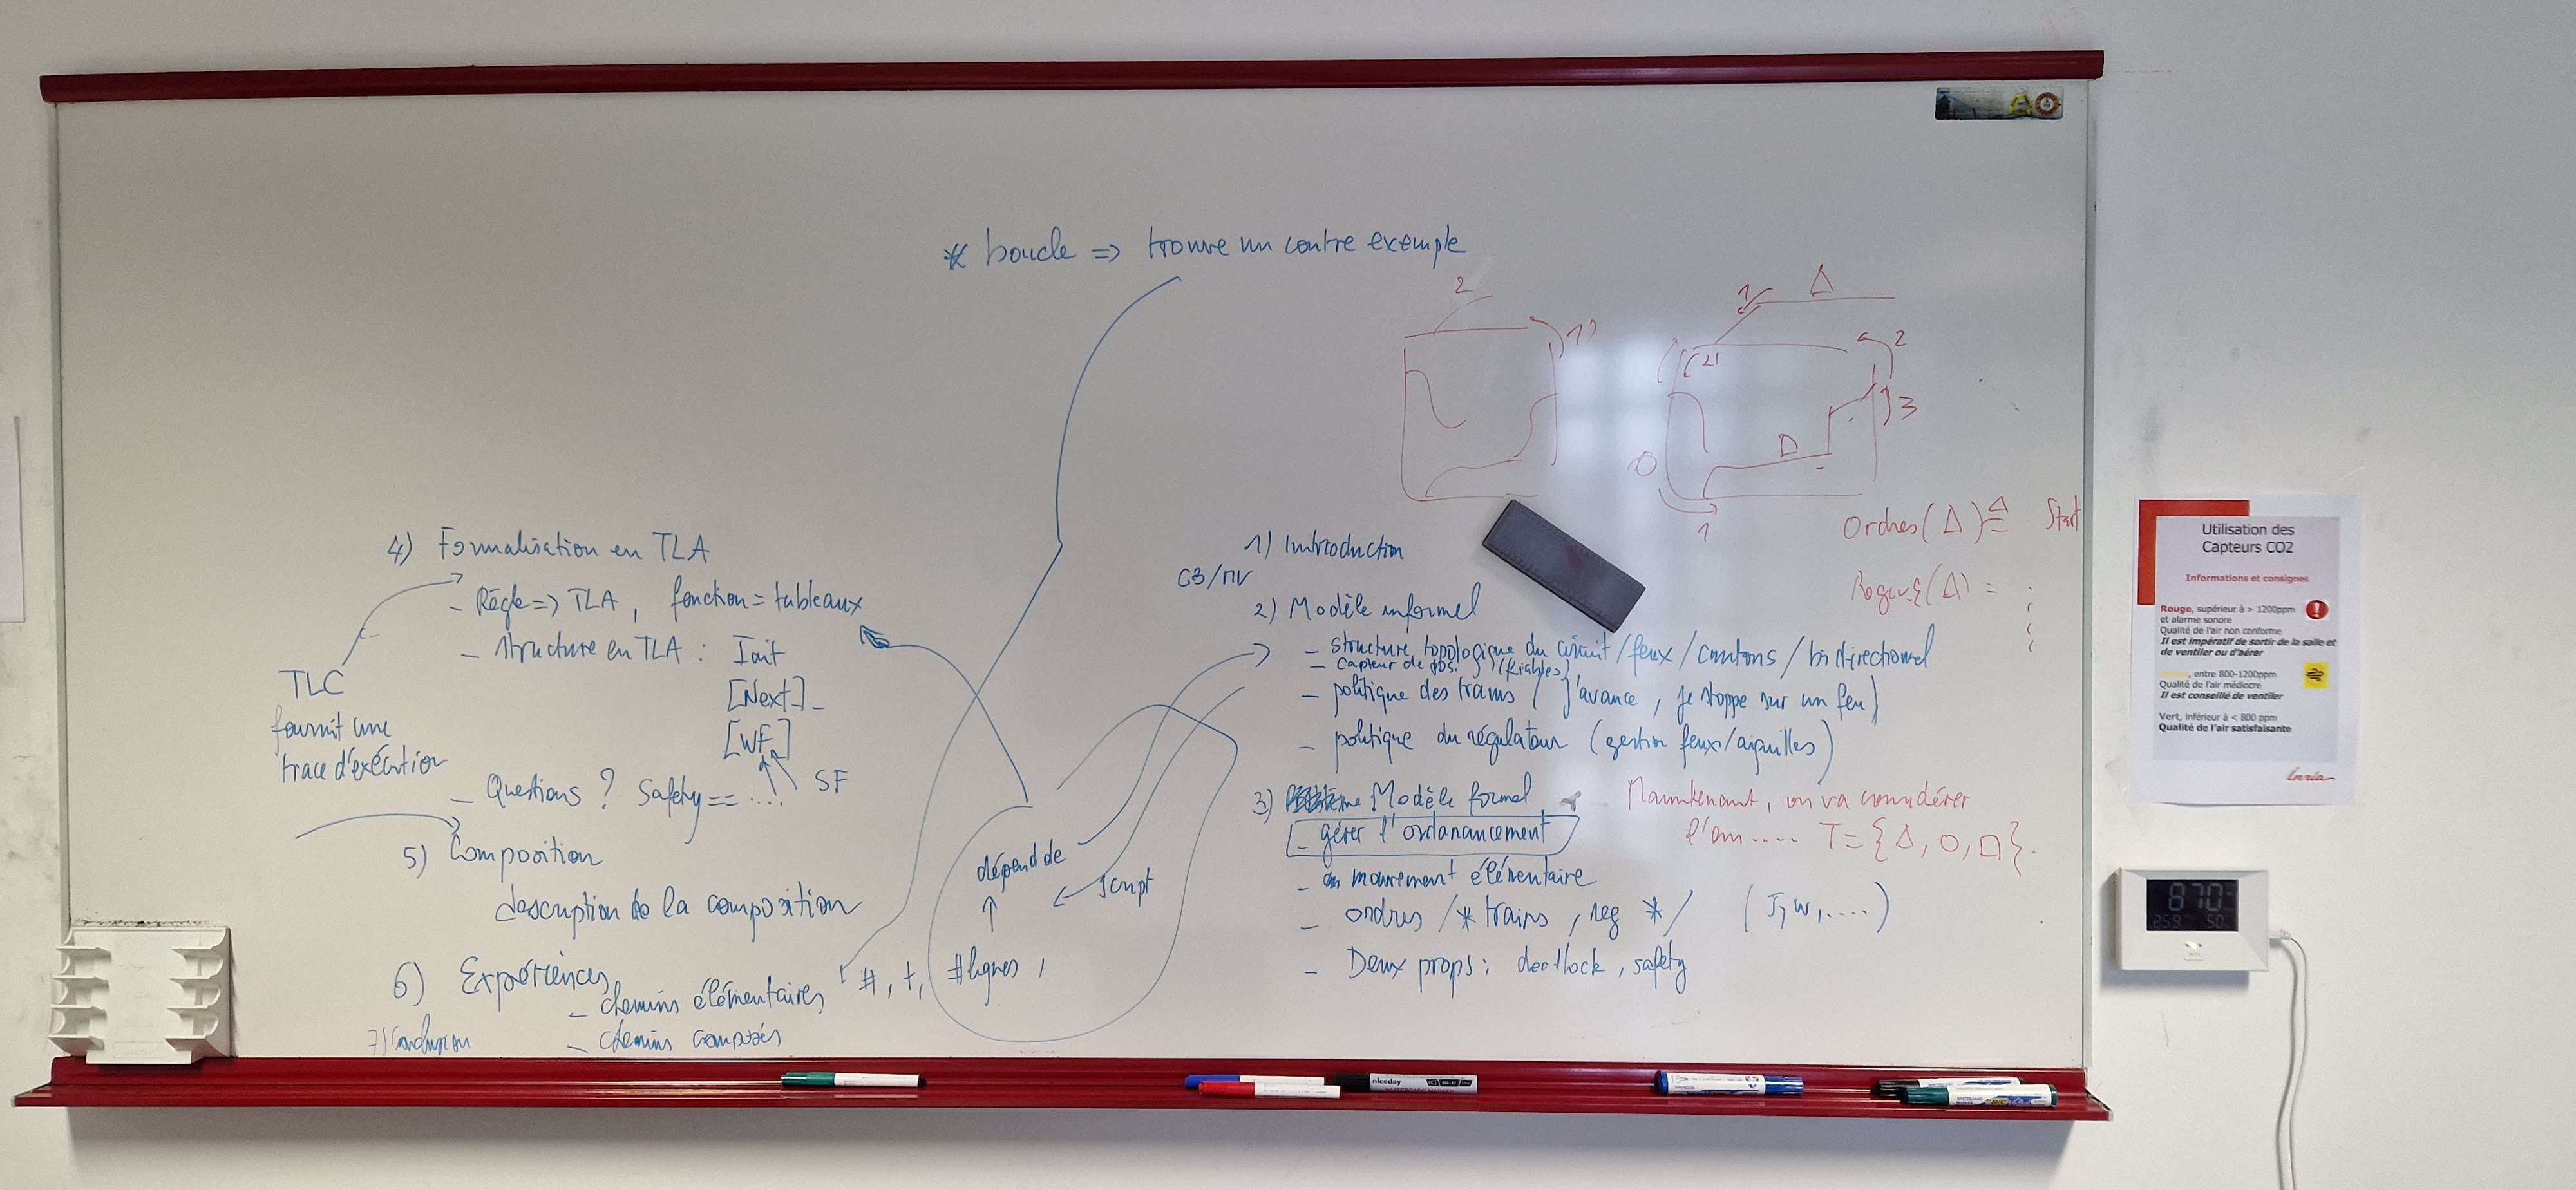
\includegraphics[scale=0.1]{img/sommaire_tableau.jpg}

\paragraph{Acknowledgements} The authors would like to thank Sébastien Schmitt from CNRS who built the train model mentioned in the introduction. That gave us a concrete reason to think about routes, scheduling and proofs. 

\bibliographystyle{splncs04}
\bibliography{refs}
\end{document}
